\chapter{Introduction}
\label{chap:introduction}

    \section{The enterprise of experimental neuroscience}
    \label{sec:introduction:neuroExp}
    This Ph.D thesis is concerned with the development of a novel methodology for studying neuronal computation \textit{in vitro}. We start with a brief overview of experimental approaches for studying this topic. Broadly speaking, neuronal computation refers to a branch of neuroscience aimed at understanding the principles by which neuronal systems generate behaviour on the basis of sensory input. This operation involves a plethora of cognitive processes such as memory, thinking, motivation, decision making, learning, consciousness etc. The current consensus within the neuroscience community is that these processes are fully realized by complex interactions between electrochemical signals in the brain and that a sufficient low level description of these is provided by classical electromagnetism and biochemistry theories. A minority view argues that such electrochemical interactions are insufficient for explaining cognitive processes and claims that further quantum descriptions will eventually be deemed necessary \cite{hameroff2014consciousness,hagan2002quantum}.

    The work of experimental neuroscience is to develop methods to accurately measure and control the spatiotemporal patterns of these electrochemical phenomena and to correlate them with behaviour. Early endeavours have focused on neurons which, owing to their excitable membrane, can transport electrical signals either actively (action potentials) or passively. Such electrical signals may be transmitted between neurons through biochemical connections (synapses) or direct electrical coupling (gap junctions). Additionally, the electrical properties of the neurons and the strength of their connections may be modified through interactions of intracellular protein and gene networks. Much of the knowledge around neuronal signalling is well established through many decades of research and considered textbook material \cite{Kandel}. Nevertheless, new modes of interaction involving novel cell types and chemical species are still being uncovered at a high pace. More recently, focus has been turned also to interactions involving non-neuron cell types \cite{volterra2005astrocytes,olah2009regulation}. This wealth of information has given rise to the field of computational neuroscience where the powers of mathematical analysis and numerical simulations as well as theories of complex systems from physics and computer science are harnessed in an attempt to bridge the gap between low level interactions and high level behaviour. To date, no comprehensive theory has emerged from these endeavours.

    Experimental neuronal computation research techniques may be broadly classified into two categories: \textit{in vivo} and \textit{in vitro}. \textit{in vivo} techniques refer to measurements and manipulations performed in living animals. The strength of this approach lies in the ability to directly correlate the behaviour of the animal with measurements performed at the same time. The importance of this capability cannot be overstated because, in a system of such complexity, making measurements without grounding them to an output could easily result in irrelevant observations. Thus, it common that results obtained in tissue sections need to be validated \textit{in vivo} before they receive full recognition. Current state of the art \textit{in vivo} techniques allow recording of action potentials from a few thousand  neurons of an identified type either electrically (electrophysiology) \cite{berenyi2014large} or optically (calcium imaging) \cite{emiliani2015all} while the animal engages in a behavioural task. A yet more impressive achievement involves optical control over the electrical dynamics (e.g., the patterns of action potential generation, also termed firing patterns) of specific populations of neurons. By employing such direct low level control researchers have even been able to influence the high level behaviour \cite{emiliani2015all}. Nevertheless, the \textit{in vivo} approach suffers from a drawback that the measurements are performed in the complete system which is typically very complicated and therefore exceedingly under-sampled. Consequently, any conclusions drawn regarding the link between the measured electrochemical patterns and the sensory input or behavioural output are normally highly speculative so \textit{in vitro} approaches are required to study aspects of the system in a more controlled manner.

    \textit{In vitro} techniques refer to measurements and manipulations performed on parts of the tissue which have been removed and maintained separately in a laboratory environment. This approach offers a greater degree of control over certain parameters and allows the study of the functionality and the input-output relationship of specific sub-circuits in isolation, thus helping to elucidate the role which they play in the original, assembled system. The ability to break down to sub components is crucial when trying to reverse engineer such an ultra complex system. Very commonly, \textit{in vitro} investigations are performed on thin slices of brain dissected out to include just the specific circuits of interest. Such slice preparations are typically used in `acute' experiments where the incubation conditions allow them to be sustained for just several hours. There is also an option to culture `organotypic' slices which, under more specialized conditions, may be kept viable for several weeks. The stringent incubations conditions, however, make it harder to perform electrophysiological measurements in this case \cite{lossi2009cell}. Another \textit{in vitro} preparation under routine use is the neuronal culture. Neuronal cultures are made by completely dissociating brain tissue from the specified brain area to obtain a suspension of the constituent cells essentially without the extracellular material. These cells are seeded onto surfaces appropriate for adherent cells and they develop over weeks to from a thin monolayer of tissue which shares certain characteristics with the native one. In contrast to slice preparations where the connectivity of the native tissue is maintained, culture preparations have completely lost the original architecture. Nevertheless, they are a natural choice for studying generic properties of single neurons and simple circuits and offer very unique advantages and possibilities.

	\section{The MEA culture model for network activity in neuronal ensembles}
    \label{sec:introduction:MEANetwork}
    The idea of extracting isolated cells from brain tissue and having them develop for long periods of time in culture has been implemented as early as the 1950's \cite{nelson1975nerve}. This approach has long been considered more suitable than the native tissue for investigation into the biochemistry, molecular biology and pharmacology of the system as well as for imaging. To accommodate neuronal cultures, as is the case with any type of adherent cell type, plated surfaces need to have undergone some form of treatment. Some of the effective treatments include heating through direct contact with a flame (only applicable to glass-like surfaces), pre-plating of other cell types to build a thin ECM layer or coating with ECM polymers such as collagen \cite{dichter1978rat}. More recently, it was reported that simpler polymers with positively charged amino residues, such as poly-L-lysine (PLL), are just as effective in promoting neuronal adhesion as the previous methods and are more repeatable by virtue of the simplicity of the coating procedure \cite{mazia1975adhesion}. PLL coating has consequently become the gold standard surface treatment. This treatment involves just incubation of the surfaces in a PLL solution for several hours. It is thought that, during the incubation period, the polymer chains become adsorbed in the surface through electrostatic interactions in a process termed `physisorption'. This process results in a complete PLL covering of the surface with the positively charged amino residues left free and available to interact with negative elements in membrane proteins, thus promoting the adhesion \cite{mazia1975adhesion}. Another polymer used for coating is polyethylene-imine (PEI). This polymer is richer in amino residues and therefore performs better the the PLL on certain surfaces \cite{wiertz2010regulation}.

    Neuronal cultures are normally prepared from embryonic tissue at later stages of pregnancy. In the case of rats, for example, brains from embryos at 15-18 days into the pregnancy usually give rise to successful preparations. However, even though the native tissue at this point already contains differentiated and electrically active neuronal circuits (e.g., \cite{easton2014genetic}), the cultured cells appear to be undifferentiated initially as they take a few days to exhibit distinct neuronal morphologies \cite{dichter1978rat}. Additionally, it was shown that by tweaking culture conditions and media formulations the plated cells may be driven to produce different cultures in terms of cellular composition (e.g., to change the neurons to astrocytes ratio \cite{morrow2001sequential}). The seeded cells are therefore sometimes referred to as progenitor cells to indicate that they are partly specialized as brain cells but not fully differentiated. Over time, the seeded progenitor cells develop dendritic and axonal arborizations and develop into various cell types with distinct morphologies. For example it is common to observe neuronal cells with `pyramidal' or `stellate' morphology or astrocytes which are flat and harder to distinguish from the background tissue \cite{dichter1978rat}. The cultures contain both excitatory and inhibitory cells and at ratios similar to those observed in the intact tissue (\(\approx10\%\) inhibitory) \cite{benson1994characterization}. The neurons develop classical excitability properties with several types of typical voltage gated membrane currents as well as synaptic connections with a variety of post synaptic receptors (e.g., AMPA, NMDA and kainate glutamate gated channels) \cite{dichter1978rat,corner2002physiological}. They were shown to have intact astrocyte-neuron communication \cite{wallach2014glutamate} and extrasynaptic neurotransmitter and neuromodulator receptors \cite{eytan2004dopamine,kaufman2012long,swanwick2006development}. Overall, the available information demonstrates that the intact tissue and the neuronal culture derived from it show a striking resemblance in cytoarchitecture and that they share many molecular structures and physiological processes.

    \subsection{Measuring network spiking activity in neuronal culture}
    Early investigations of electrical activity in neuronal culture and mainly relied on intracellular recordings, i.e., electrodes inserted directly into the cytoplasm thus measuring the intracellular potentials. This technique directly measures the potential across the cell membrane and produces very large signals in the range of tens of \(mV\) with high signal to noise ratio (SNR). However, as such techniques require manual interfacing with every recorded cell, they are particularly ill-suited for concurrent monitoring of multiple cells or for long term recordings. In 1957, Hubel \cite{hubel1957tungsten} reported that thin metallic wires inserted into cats' spinal cord are able to sense sharp potential fluctuations (later termed spikes) in synchrony with the occurrence of an action potential in nearby neural cells. These extra-cellular (EC) spikes are thought to be produced by local ionic currents running in the vicinity of the cellular membrane during an action potential. As these currents are free to spread over the large volume of extra-cellular space their density around the electrode is small. This allows sensing of EC-spikes only in close proximity to neurons with relatively small amplitudes of tens of $\mu V$ \cite{herzog2011optical}. Despite these limitations, EC recordings are relatively easy and non-invasive and thus readily support long term and multi-cell recordings. Nevertheless, their utility was not accessed until many years later as technological advancement in micro-lithography allowed production of microelectrode arrays (MEAs)\cite{Morin2005,Buzsaki2004}. These devices have been used extensively both in vitro and in vivo to study neuronal activity in various neuronal systems. Specifically in the context of neuronal cultures a planar MEA is used where the electrodes are embedded in the surface. Neurons are seeded onto the surface and thus interface with the electrodes naturally during their development\cite{PotterRev2001,Morin2005,Marom02}.

    A significant body of work was dedicated to characterizing the spiking activity of neuronal cultures grown on MEAs. The cultures start showing spontaneous action potential activity (spiking) as soon as a few days \textit{in vitro} \cite{wagenaar2006extremely,kamioka1996spontaneous}. The spiking is variable in form but tends to show increasing synchrony across all recording electrodes as the culture matures. Typically, the activity organizes into short periods of `network bursts' lasting 100-200 ms during which intense firing is observed across all the electrodes. Over development, the spiking and bursting activity are known to increase for about 3 weeks before somewhat declining and finally reaching a plateau \cite{chiappalone2006dissociated,bikbaev2015brain,kamioka1996spontaneous}. These changes to the activity seem to align with the development of excitatory synapses whose density follows a similar time course \cite{li2003some,ramakers1994activity}. Inhibitory transmission in cultures was also studied specifically and shown to follow a characteristic time course. Inhibitory synapses appear in delay as compared to excitatory ones and are preceded by appearance of GABA membrane receptors uniformly spread in extra synaptic areas. These receptors gradually become concentrated in synaptic structures but it is not before 3-4 weeks \textit{in vitro} that such GABAergic synaptic structures become prevalent \cite{swanwick2006development}. This delayed development of GABAergic transmission is strongly manifested in the observed patterns of spiking activity on the MEAs. The network bursts are initially long and diffuse and narrow down as the cultures mature \cite{van2004long,wagenaar2006extremely,bikbaev2015brain}. Additionally, younger cultures at the 2\textsuperscript{nd} and 3\textsuperscript{rd} weeks tend to exhibit periods of continuous epileptiform like discharges which take the form of numerous network bursts occurring at close temporal proximity and are therefore sometimes termed `superbursts' \cite{wagenaar2006extremely}. The noted observations suggest that the excitatory and inhibitory transmission develop over different time courses and that the mature excitation-inhibition balance is obtained only at 4\textsuperscript{th} week \textit{in vitro}. Interestingly, this developmental time course is conspicuously similar to the time course of the critical period in rat pups which is the time frame just following birth during which the nervous system is known to undergo experience dependent organization \cite{hensch2004critical}. This organization is known to involve synaptogenesis as sensory neurons establish links with their downstream targets followed by activity dependent pruning. These processes seem to be present in the development of neuronal culture which could therefore serve as an interesting, as of yet unexplored, model for the dynamics of the critical period.

    Over the previous century, neuronal cultures were the method of choice for neuroscience investigations due to the accessability that they provide to basic biochemical and biomolecular elements. However, with the technological advancement of \textit{in vivo} techniques where neuronal activity can be recorded in behaving animals, neuronal cultures began to be regarded as irrelevant in the context of neuronal computation. Additionally, neuronal culture systems have been criticised for being fundamentally different from the respective native tissue, e.g., showing a different genetic makeup, making it very hard to make comparisons and draw relevant conclusions. Indeed, since even the basic principles of neural computations in the real brain have not been established, it is unclear to what extent they have been compromised in the transition to culture. Nevertheless, from the ethical perspective, neuronal cultures comprise the neuroscience experimental platform which involves the lowest levels of animal suffering and it is actually the most relevant one for certain research questions that involve generalized properties of neurons. Examples for such studies are reviewed next.

    \subsection{Notable achievements and advantages of neuronal cultures on MEAs}
	\label{sec:introduction:achievements}

    The Potter group used neuronal cultures to study the principles of synaptic scaling \cite{fong2015upward}. Synaptic scaling is a homeostatic mechanism which modifies the strengths of the synapses to prevent synaptic currents from becoming too extreme. Learning is thought to involve behaviour dependent modifications to synaptic strengths (plasticity). Thus scaling probably affects learning and is therefore important computationally. They applied synaptic blockers to the cultures which would normally cause the spontaneous activity to vanish and consequently induce synaptic up-scaling (strengthening). However, using optogenetic control he was able to artificially restore the normal activity patterns in the entire culture without the involvement of the synapses (figure \ref{fig:introduction:MEAAch}A1). In this way, a decoupling of the spiking activity from synaptic activation was achieved. The main finding was that, in the presence of synaptic blockers, the same level of up-scaling was observed, regardless of whether the cultures were active (artificially, through the optogenetics) or silent (figure \ref{fig:introduction:MEAAch}A2). This demonstrates that the scaling process directly senses synaptic activation rather than the global spiking activity of the cell. This finding has bearing to computational modelling of plastic neuronal systems.

    An influential neuroscience work from 1995 showed that single neurons produce an unreliable spiking output when presented with constant current input but become exquisitely accurate in the face of white noise input which better mimics synaptic drive \cite{mainen1995reliability}. These data were originally used to argue that neurons may support `spike timing' type of coding. In a recent series of seminal studies, the Marom group used neuronal culture to take these ideas further \cite{gal2013entrainment,gal2010dynamics,reinartz2014synaptic}. They applied synaptic blockers to neurons grown on MEAs so as to render them functionally isolated. MEAs make it is easy to quickly accumulate recordings from many neurons under controlled input. They found that the neurons were indeed unreliable under a constant stimulation pattern but even under a white noise pattern their apparent reliability was short lived. On the other hand, when a stimulation signal with a power law correlation structure (which resembles natural type input) was used, the neurons followed it accurately for extended periods of time. Power law correlations mean that the signal at hand contains random processes at a wide range of time scales, from milliseconds to hours (figure \ref{fig:introduction:MEAAch}B). The results demonstrate that individual neurons possess the ability to code processes at a variety of behavioural time scales. This notion contradicts common assumptions in the field that time scales of a single neuron are relatively fixed and that slower behavioural processes emerge strictly out of network interactions.

    The Moses group used conditions where the synapses were blocked from the pre-synaptic side which means that the synaptic tone is maintained but not the fast phasic transmission between the neurons \cite{penn2016network}. Under these conditions they found that the disconnected neurons establish a spontaneous firing pattern each with a characteristic rate (figure \ref{fig:introduction:MEAAch} C). They also found that the original firing rate of the whole network prior to the disconnect was roughly the average of all the individual unit rates. This work shows an important interplay between the properties of the units and the properties of the network and demonstrates the important role that intrinsic excitability plays in the network dynamics.

    \begin{figure}[!htb]
        \centering
        \includegraphics[width=14cm]{chapter1/figures/MEAAchievements/MEAAchievements.png}
        \caption[Examples studies demonstrating the utility of neuronal culture based research system]{\textbf{The neuronal cultures on MEA platform has provided an unprecedented level of control over experimental parameter} (A1) Fong et. al. established a feedback system whereby the spiking activity was continuously monitored on the MEAs. As soon as it decreased below a threshold an optogenetic activation was administered to the entire culture. This system was used to keep the spiking activity levels stable despite a pharmacological blockade of the AMPA receptors. (A2) Sample intracellular voltage traces recorded following 24 hours of control treatment (top) or of CNQX blockade of AMPA receptors without (middle) or with (bottom) optogenetic stimulation to maintain levels of spiking activity. Averaged EPSP waveform in each of the above conditions is shown below the voltage traces. 24 hours of CNQX blockade results in the same level of synaptic scaling (increase in EPSP amplitude) regardless of whether spiking activity levels were artificially maintained.}


    \end{figure}
    \clearpage


   \begin{figure}[!htb]
        \captionsetup{labelformat=adja-page}
        \ContinuedFloat
        \caption[]{(B, left) Firing rate plots of a neuron in response to 10 identical stimulations sequences, under three different stimulation regimes: Constant inter-stimulus intervals (top), inter-stimulus intervals which constitute a white noise process (middle), inter-stimulus intervals which constitute a scale free (1/f) process (bottom). The stimulation rates are shown in black and the neuron responses to the repeated stimuli presentations are overlayed in color. Reponses to the constant interval stimulation show no reproducibility at all. Responses to the white noise show reproducibility over shorter time scales (inset) but not over longer ones whereas responses to the scale free input show reproducibility over all time scales. The reproducibility is further demonstrated in the pairwise distance matrices (right) which show distances between responses to presentation of identical stimulation sequences. The distances was computed as 1 minus the correlations between the respective responses. (C) Network raster plots and their summation under decreasing levels of extracellular Ca\textsuperscript{2+} which inhibit the synaptic function. At low levels of synaptic coupling the neurons exhibit spontaneous spiking activity each with a characteristic firing rate. At high levels of coupling the neurons tend to fire only within the confines of network bursts. The mean firing rate is unaltered across the conditions (not shown here). This data shows that the neurons inherently regulate their firing rate and that, upon coupling between the units, this individual activity set value is a determinant of the network burst rate. The data shown in this figure is adapted from \cite{fong2015upward}, \cite{gal2013entrainment} and \cite{penn2016network} with permission.}

        \label{fig:introduction:MEAAch}
    \end{figure}

    The studies reviewed above all uncovered fundamental properties of neuronal computation at the single cell and network level. These studies could only have been performed \textit{in vitro} because of the required control over the connectivity and the input. Moreover, neuronal culture is the most natural platform for these types of experiments because they are concerned with generic properties of neuronal systems regardless of a specific architecture. These examples demonstrate that many low level properties of the system are yet to be uncovered and highlight the importance of the control offered by neuronal culture for accessing these properties. Another important control feature available strictly with neuronal cultures is that of the architecture. All other experimental platforms (including slices) are limited to the native architecture. This may be limiting when trying to understand the importance of the physical architecture of a circuit to the specific computation it performs. The fact that that neuronal cultures develop from the very basic elements, i.e., dissociated cells, has made it possible to design bespoke circuits and therefore has offered a fresh approach to studying the structure-function link in a controlled manner. Photolithographic techniques have been applied to generate surfaces with patterned adhesive or repulsive polymer coatings. These have been used to study how a modular organization at various levels of hierarchy affects the neuronal dynamics \cite{levy2012enhancement,shein2011engineered}, to generate highly ordered networks at near single cell resolutions \cite{kwiat2012highly,kang2010generation} and to control the patterns of electrical propagation \cite{feinerman2008reliable}. Microfluidics technology, which can produce closed compartments with micro-scale features and with separate access ports has allowed the generation of modular networks with mixed populations and with directional connectivity thus modelling interactions between separate brain regions \cite{robertson2014chemically,honegger2016microfluidic,peyrin2011axon,dauth2016neurons}.



    Another aspect of neuronal circuits that can be readily manipulated within neuronal cultures but is harder to access in other systems is the extracellular environment. As described in section \ref{sec:introduction:neuroExp}, computation in neuronal tissue is performed via complex spatiotemporal patterns of electrochemical interactions. These include fast electrical signals that propagate through the tissue as well as an abundance of chemical signals, both intra- and extra-cellular, that interact with each other and with the electrical ones. Due to the nature of technology, it has been historically easier to interface with the tissue electrically rather than chemically. As a consequence, the experimental toolbox and the accumulated knowledge has been strongly biased towards the electrical signals. However, these are just a small part of the relevant interactions that comprise the action of the tissue. In recent years, novel research initiatives together with the development of chemical sensors have started to uncover principles of the extracellular chemical signalling. Such processes are the concern of this Ph.D work.

 


    \section{Volume transmission in neuronal systems}
    \label{sec:introduction:volTrans}
    The Reticular Theory, mainly attributed to Camillo Golgi, was the first attempt to provide a description of how information is encoded and propagated through brain tissue. It advocated that the brain essentially comprises a single continuous compartment where chemical species are free to travel in all directions via diffusion. According to Golgi, the complex spatiotemporal patterns formed in this space are enough to account for brain function. The reticular theory was made obsolete upon the discovery, by Ramon Y Cajal, that the brain is mainly made out of discrete and separate elements, the brain cells, and the establishment of the Neuron Doctrine. Over the years, it has become well established that the neurons form a network that supports a highly specific and rapid point-to-point mode of communication where information travels as electrical signals within the cells and is transmitted between them through synapses and gap junctions. These specialized communication elements are designed to transmit signals specifically between pairs of cells. This type of architecture is considered the main substrate of information processing in the brain and has inspired important ideas and applications in machine learning and artificial intelligence. Nevertheless, in recent years it has become clear that, to a large degree, communication between cells in the brain is also mediated by secretion and sensing of chemical species in the extra-synaptic space and that these types of interactions are required to account for some of the observed functional properties of the system \cite{agnati1995intercellular,fuxe2010discovery}. Ironically, these types of interactions are similar to those originally proposed by the Reticular Theory because the extrasynaptic space may arguably be regarded as a single large compartment without a particular directionality of information transfer. Typically, signaling molecules that are released in the extra-synaptic space are free to diffuse in all directions in the surrounding volume of tissue and would therefore influence all the cells residing in that volume. This mode of communication has been termed volume transmission (VT) to account for its spatial characteristics and its lack of specificity. Correspondingly, the precise communication that proceeds along neuronal membranes and between designated cell pairs is referred to as wired transmission (WT).

    \begin{figure}[!htb]
        \centering
        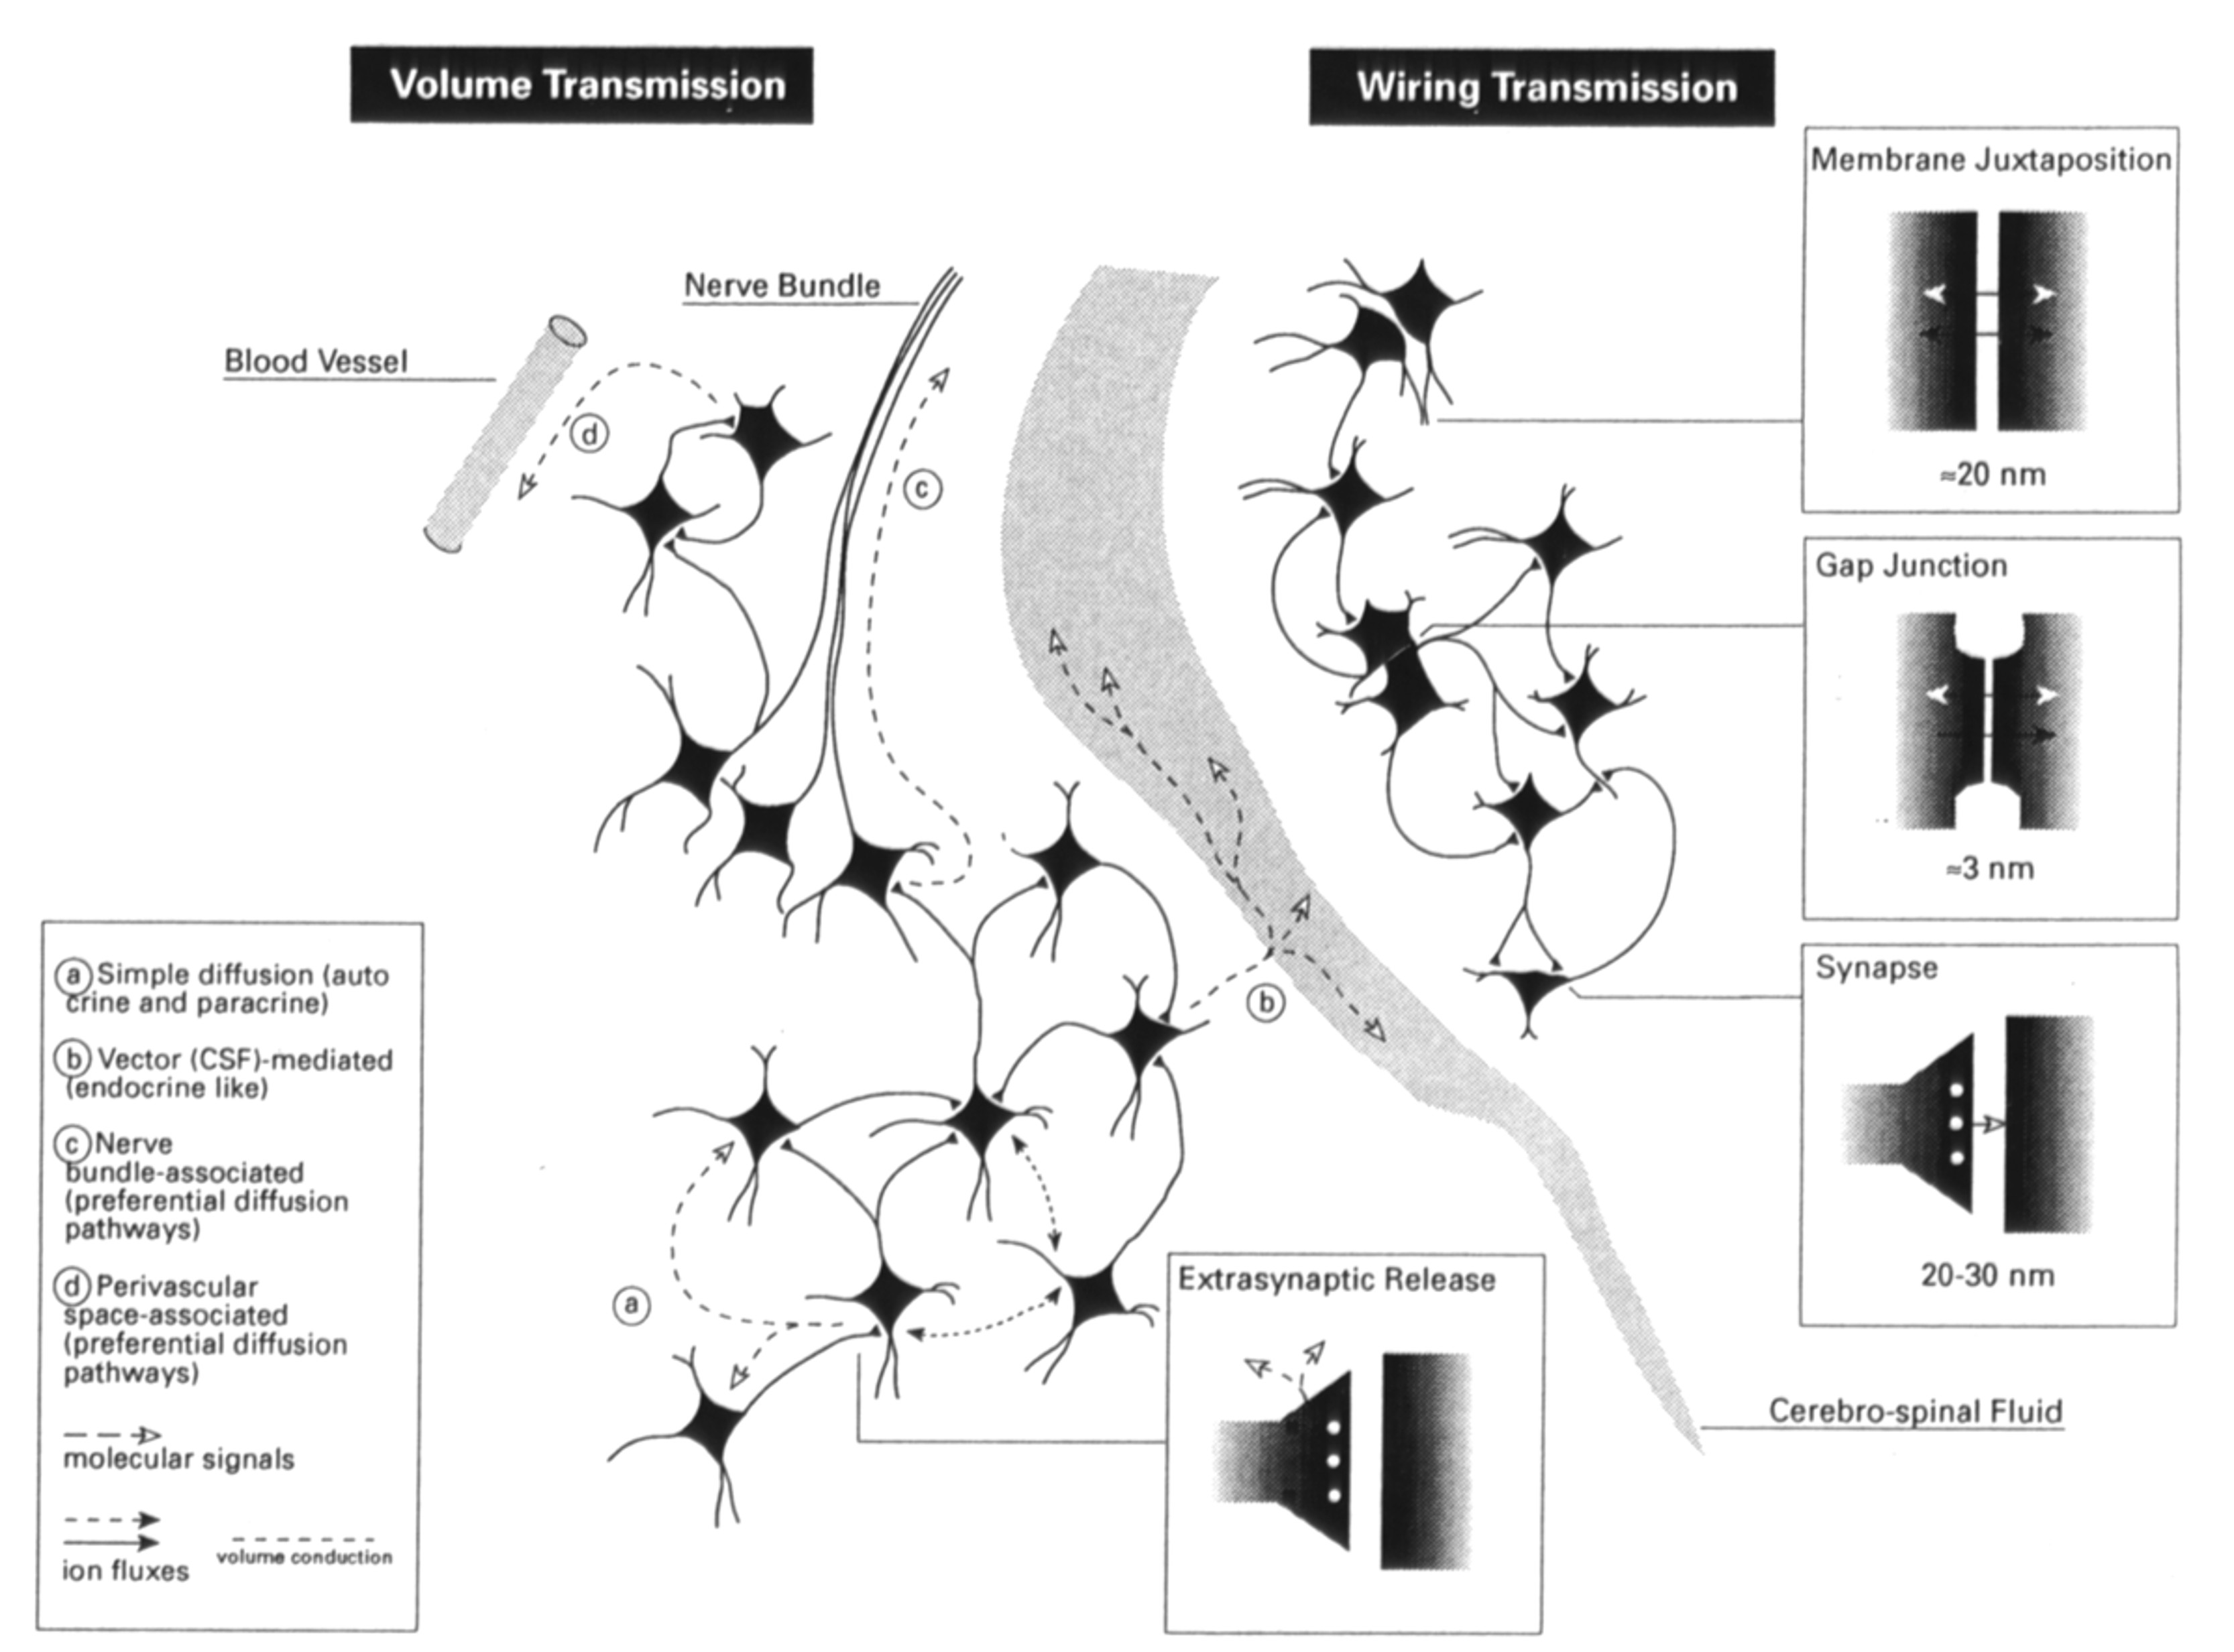
\includegraphics[width=14cm]{chapter1/figures/volTrans/volTrans.jpg}
        \caption[Illustration of the volume and wired transmission concepts]{\textbf{Illustration of the volume and wired transmission concepts.} Wired transmission operates between well defined cell pairs and mainly mediated through synapses although other structures have also been implicated (gap junctions and membrane juxtapositions). Volume transmission operates unspecifically on cell populations and is mainly mediated via diffusion in the extrasynaptic space. CSF transport and interstitial flow have also been identified as mechanisms for conveying molecular signals. Adapted with permission from \cite{agnati1995intercellular}.}
        \label{fig:introduction:volTrans}
    \end{figure}

    As stated above, VT is mainly associated with signalling molecules secreted by the source cells and sensed by the receiving ones. Nevertheless, other types of non-specific interactions have also been included in the VT family. These include interactions between ECM proteins in a `global molecular network', electrical induction between neurites (also termed ephaptic interactions) and blood pressure driven stretching of the brain tissue \cite{agnati2006volume}. Recently, it was shown that changes to the ionic composition of the extra-cellular space underlies the transition between sleep and wakefulness \cite{ding2016changes}. Such control of the the ionic concentration may also be categorized as VT.

    In the context of the system proposed in this work, we propose to categorize classical VT (i.e., VT operating via signalling molecules diffusing in the extra-synaptic) into two groups: intrinsic and extrinsic VT. Intrinsic VT refers to processes where the source cells are within the target tissue. Notable species participating in intrinsic volume transmission are GABA and glutamate. These neurotransmitters are primarily known for their role in excitatory and inhibitory WT. However, over recent decades, it has become widely recognized that many of the receptors for these transmitters, both ionotropic and metabotropic, are located at extrasynaptic locations thereby implying an ambient presence of their agonists \cite{farrant2005variations,taber2014volume}. GABA and glutamate arrive at the extrasynaptic space through a wide variety of secretion processes including synaptic spillover \cite{matsui2003ectopic,hamann2002tonic,bellamy2006interactions} and direct release through specialized transporters in neurons \cite{cavelier2005tonic}, astrocytes \cite{lee2010channel,cavelier2005DIDS} and the newly identified neurogliaform cells \cite{olah2009regulation}. All these release mechanisms dynamically operate in feedback from the activity in the network and have been implicated to be involved in information processing \cite{mann2010control,hamann2002tonic,lenk2016understanding,cavelier2005tonic}. Other well characterized species involved in intrinsic VT are adenosine \cite{wall2015localized}, ATP \cite{zhang2003atp}, endocannabinoids, neurosteroids and nitric oxide \cite{fuxe2010discovery,bellamy2000rapid} which almost all operate through specialized membrane receptors and are released from neurons and astrocytes across the nervous system. Nitric oxide is an exception as it readily crosses the cell membrane without mediation and directly operates on intracellular targets.

    Extrinsic VT refers to processes where the source cells are located outside the target tissue. Typically, these signals originate in specialized nuclei with neurons capable of producing the designated signalling molecules. These neurons innervate the target tissue and the signaling species are secreted by means of vesicle release. Since the release mechanisms employ pre-synaptic machinery it was long thought that extrinsic VT was actually WT. However, today it is well recognized that these long range nerve terminals do not form full fledged synaptic structures in the target tissue because the presynaptic machinery is typically not matched with a post synaptic receptor density \cite{taber2014volume,rice2008dopamine}. Similarly to intrinsic VT, a large proportion of membrane receptors associated with extrinsic VT signals are uniformly spread in the tissue. An extreme form of this organization is seen in the neuropeptide VT systems which include substances such as neurokinin, \textbeta-endorphin, cytokines and oxytocin \cite{fuxe2010discovery,veening2012volume}. Membrane receptors associated with these substances have been shown to exist in brain regions which are apparently not innervated by the neuropeptide producing nuclei. Indeed these substances have been shown to travel long distances in the brain, in part using the CSF, to reach the non-innervated areas and their presence in the tissue is sustained for hours following the release events. The other major family of extrinsic VT signals are the central monoamines, usually referred to as `neuromodulators' and which include dopamine (DA), acetylcholine (ACh), noradrenaline (NA), serotonin (5-HT) and histamine. The neurons producing these monoaminergic signals are located in distinct nuclei in the brain stem and basal forebrain and all show a similar organization in that they project quite densely to the entire brain \cite{gu2002neuromodulatory}. Since the rate of release and re-uptake depends on the density of pre-synaptic sites, the dense innervation pattern of these systems means that they are capable of producing rapid phasic volume signals. These systems are the topic of the next section.



    \subsection{Neuromodulator transmission and plasticity}
    The ascending neuromodulatory pathways have been drawing increasing levels of interest within the neuroscience community. Their anatomic organization is similar in that they all innervate the entire forebrain although the precise innervation pattern varies between the systems in a species specific manner \cite{gu2002neuromodulatory}. All the neuromodulators are also strongly involved in wake-sleep cycling and their levels in the forebrain decrease during sleep and increase upon awakening \cite{saper2005hypothalamic}. These systems, and particularly the dopaminergic, cholinergic and noradrenergic ones, have been shown to be important for plasticity and therefore hypothesized to be involved in cognitive processing. Their role in plasticity was first observed in classical sensory deprivation experiments where suturing one eye or denervating certain afferent somatosensory nerves would cause a reorganization in the associated cortical tissue. Damage to the neuromodulatory systems impaired these reorganizations \cite{gu2002neuromodulatory}. These three systems were also shown to affect classical \textit{in vitro} plasticity experiments where LTP or LTD are induced through controlled stimulation in paired neuronal populations. Presence of neuromodulators in the bath during such experiments have been shown to have a gating effect on the plasticity or to change the direction of the observed change \cite{zhang2009gain,yagishita2014critical,huang2012pull,otani2015dopaminergic,isaac2009hippocampal}. Correspondingly, a strong involvement of these systems was demonstrated also in behaving adults animals engaged in learning tasks. Learning is impaired by damaging these systems or gated through optogenetic control of the relevant nuclei \cite{tsai2009phasic,ogren1980evidence,hasselmo2006role}. Beyond the established role in plasticity and learning, the neuromodulators have been shown to have an acute direct effect on the activity of the network in various forebrain regions both \textit{in vitro} \cite{eytan2004dopamine,kaufman2012long,otani1998dopamine,gu2002neuromodulatory} and \textit{in vivo} \cite{tye2013dopamine,carter2010tuning,kuchibhotla2017parallel}. These changes to network dynamics have been linked to context dependent modulation of sensory processing and of behaviour. The context information provided by the modulators has been interrogated through subjecting laboratory animals to behavioral tasks while monitoring the activation patterns of the respective nuclei. Dopamine has been found to mostly convey reward and novelty information but to a certain degree also salience \cite{schultz2013updating,bromberg2010dopamine}. Acetylcholine seems to be related to conscious attention and salience \cite{pinto2013fast}. Noradrenaline has been the least studied of the three but is definitely associated with motivation and arousal \cite{carter2010tuning}. Overall, these neuromodulator systems seem to convey different but somewhat overlapping contextual information and this is used by other parts of the brain to modify behaviour accordingly and to learn the necessary associations.

    Further recent developments have provided new information as to how the neuromodulator information may be used to generate the correct associations at the circuit and synapse level. This pertains mainly to the observation that discrete rewarding events during behavioural tasks (e.g., the monkey receives a peanut) are associated with a sharp burst in the dopaminergic nucleus (VTA) and an accompanied phasic increase in the dopamine concentration in target tissue which lasts for no more than a few seconds \cite{schultz1997neural,venton2003real,arbuthnott2007space}. Given these sensor measurements and the highly extrasynaptic distribution of dopamine receptors in the tissue \cite{rice2008dopamine,taber2014volume} (also see figure \ref{fig:introduction:extVolTrans}) it seems that these are truly volume signals and therefore are not specific to a particular cell or synapse. Moreover, taking into account the significant divergence in projections from the dopamine nucleus to the rest of the forebrain, it is likely that large portions of tissue receives the same dopamine signals in synchrony. This low level of spatial but high degree of temporal specificity seem to be compatible with the notion of reinforcement learning where the reward signal does not carry in itself specific algorithmic information as to how to perform the task but the temporal presence of reward or lack thereof is implicitly used to modify the circuit appropriately. The discovery of this mode of operation for dopamine was followed by similar observations for Acetylcholine \cite{sarter2009phasic} and noradrenaline \cite{dugast2002vivo}. Thus, it is possible that all these neuromodulators support reinforcement learning based on the contextual information that they carry. These observations have spurred a vibrant debate in computational circles about how to reconcile previously described neuronal plasticity rules with the novel observations about neuromodulators. These are reviewed next.

    \begin{figure}[!htb]
        \centering
        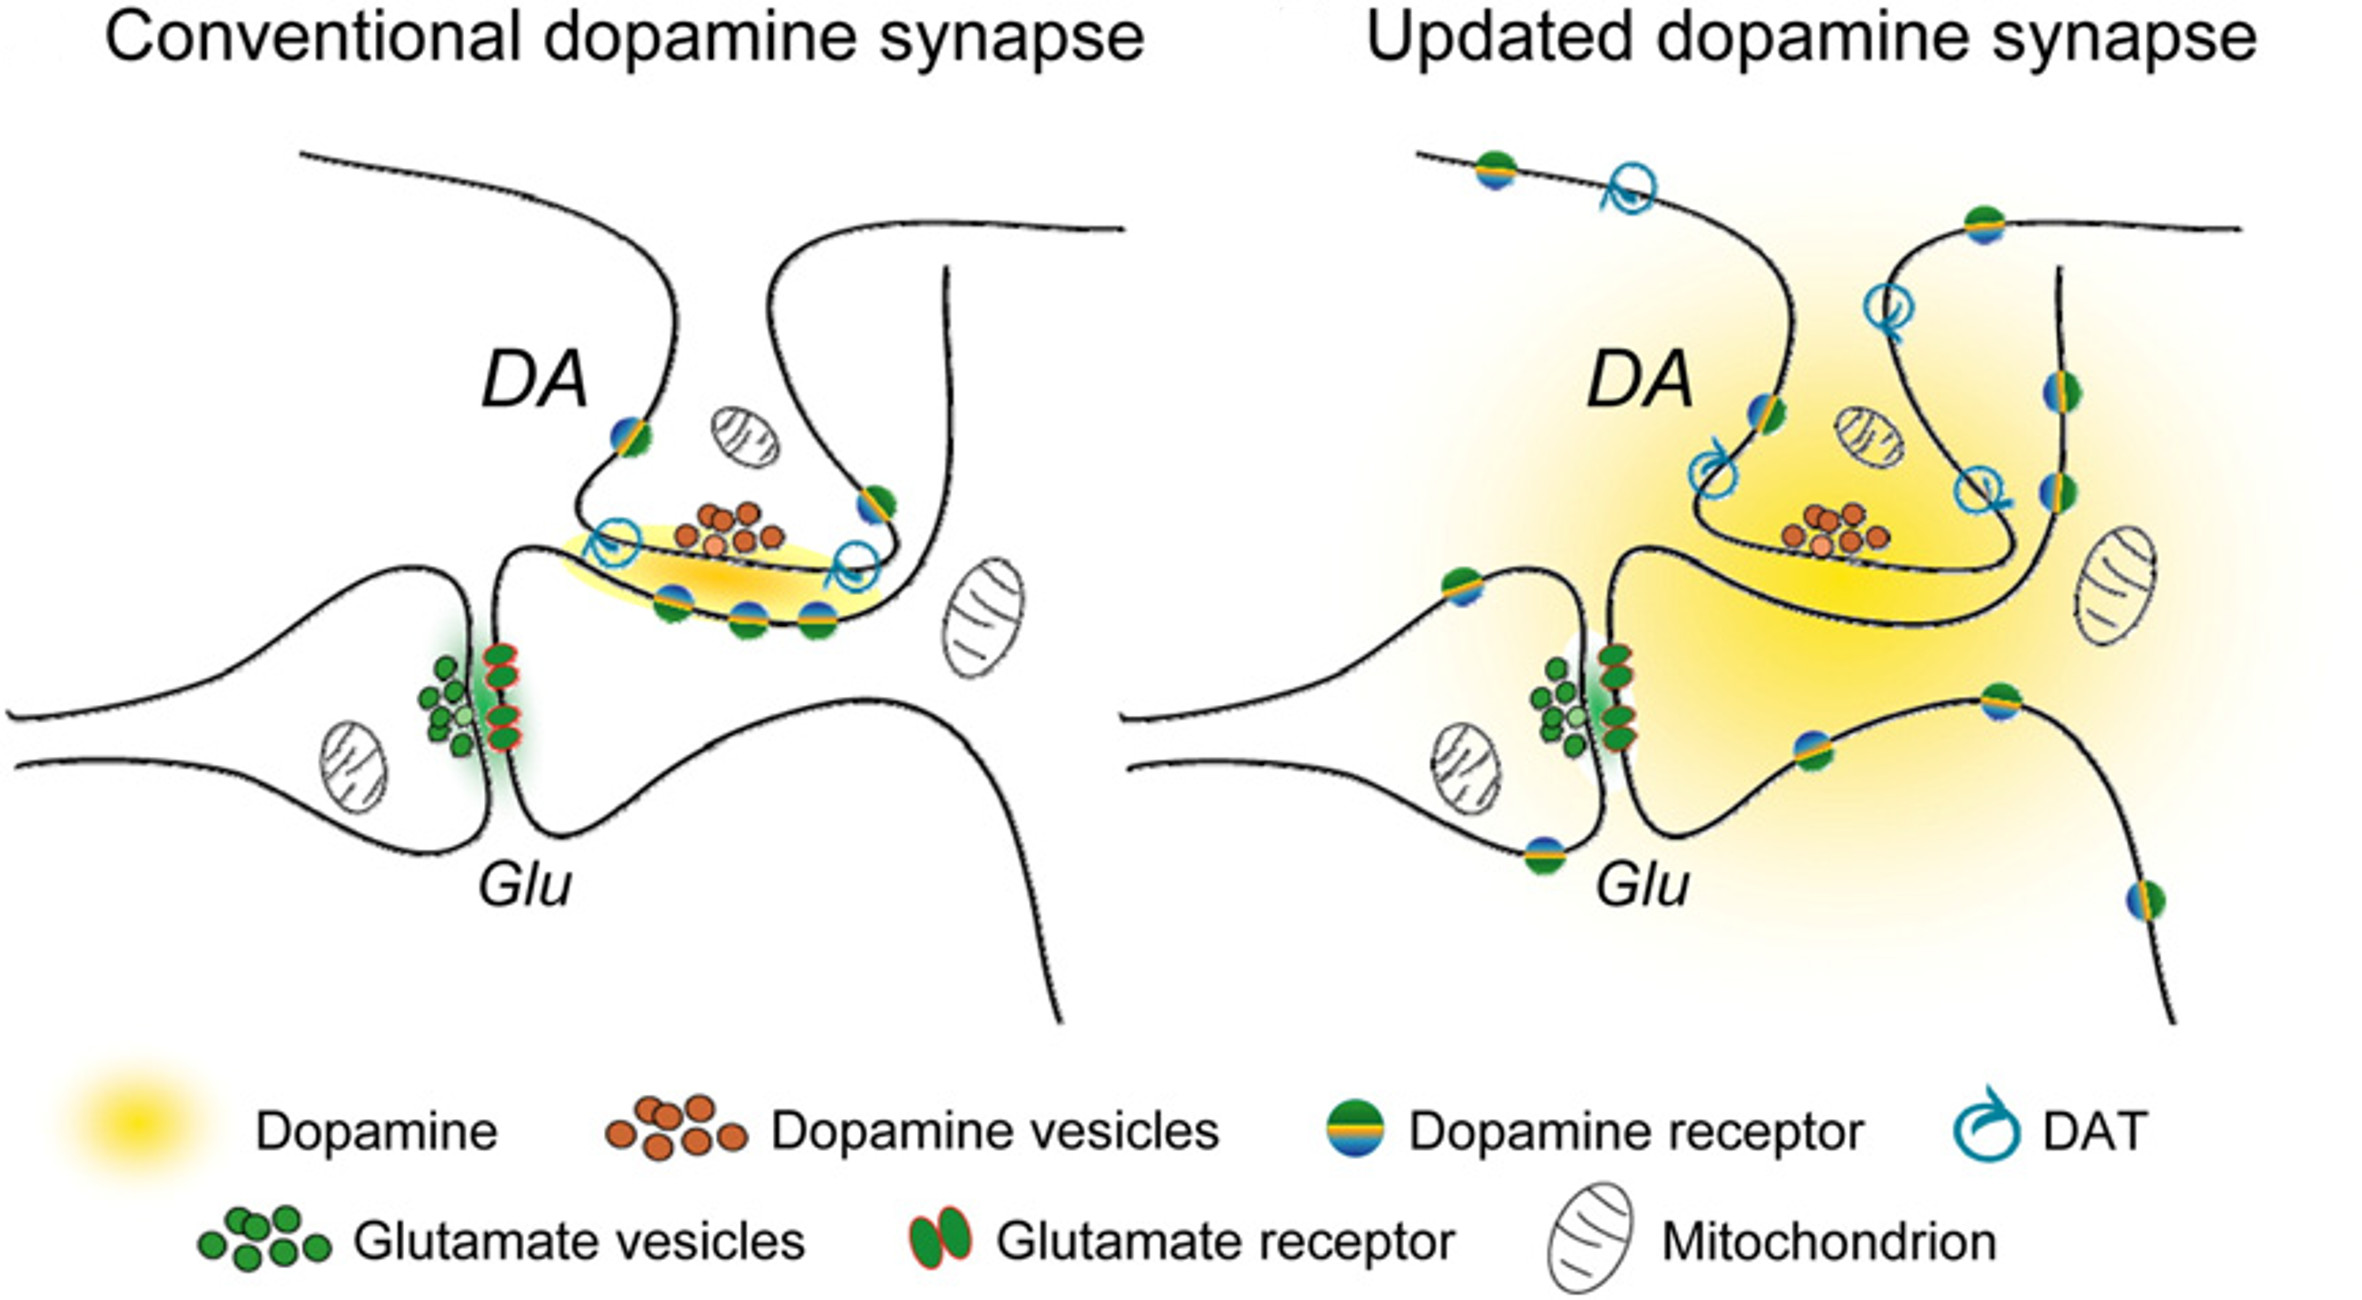
\includegraphics[width=10cm]{chapter1/figures/extrinsicVolTrans/extrinsicVolTrans.jpg}
        \caption[Volume transmission view of dopamine signalling]{\textbf{Dopamine operates as volume signal.} Dopamine and other monoamine signalling pathways have been previously considered to operate via classical synaptic transmission because they are released from nerve terminals. Recent immunocytochemistry work demonstrates that a large degree of mismatch between the locations of monoamine release sites and their respective receptors. This mismatch is taken a evidence that these systems operate in volume transmission mode. Adapted with permission from \cite{rice2008dopamine}.}
        \label{fig:introduction:extVolTrans}
    \end{figure}

    \label{sec:introduction:neuromodulators}
    \subsection{The Izhikevic thought experiment}
    For many years, since the influential work of Donald Hebb \cite{hebb1961organization}, neuroscience had essentially just a single learning rule at its disposal. That was the Hebbian plasticity rule which states that ``neurons that fire together, wire together''. This originally hypothetical concept was later proven experimentally \cite{bliss1973long}. This rule was later adjusted to account for the need to also reduce the strength of connection and to align with various experimental observations \cite{caporale2008spike,bi1998synaptic}. One of the generally accepted forms of this rule is the spike timing dependent plasticity (STDP) which asserts that a synapse would be strengthened when the presynaptic neuron had fired shortly before the post synaptic one. Alternatively it would get weakened if the temporal coupling had been reversed. The correlations required for this form of plasticity are variable but are generally in the order of tens of milliseconds. This form of plasticity is well established experimentally \textit{in vitro} and has been able to account for some connectivity features observed in the nervous system. However, making computational models of higher level learning and memory is difficult when using it on its own \cite{brea2016does}. Incorporation of reinforcement learning principles in computational theories has allowed generation of models of episodic and associative memory \cite{brea2016does} and even of goal directed behaviour that requires learning \cite{brea2016does,fremaux2013reinforcement}. Thus the notion of a neuromodulator carried reinforcement signal is a major step forward in the theoretical understanding of cognitive processing. The computational work in this context usually assumes the presence of a low level mechanism whereby the classical STDP rule is modulated by the concentration of dopamine so as to allow plasticity to occur at the appropriate part of the circuit. Several forms of this mechanism have been suggested (reviewed in \cite{fremaux2015neuromodulated}) and we will next present one prominent example for such a formulation, suggested by Izhikevich \cite{izhikevich2007solving}.

    Izhikevich was concerned with the fact that rewarding events in the real world are a product of behaviour (e.g., a toddler trying to open a box of candy) and  therefore operate at very different time scales and usually arrive in delay as compared to the neuronal activation pattern that generated them. The question of how to link variable rewarding events to preceding neuronal activation is sometimes termed the `distal reward problem'. Izhikevich suggested thats STDP events, i.e., spikes occurring in both the pre- and post- sides of a synaptic pair at close temporal proximity, do not immediately elicit plasticity as originally formulated in the STDP principle, but actually initiate an `eligibility trace' which decays at a time constant of several seconds. The activated synapse would then only be reinforced if a dopamine flux arrives before its eligibility trace has decayed completely (figure \ref{fig:introduction:izhi} A-C). Based on this principle, a rewarding event would reinforce all the synapses that participated in preceding spiking activity within the eligibility trace time scales. This may mean that synapses that have been active by chance due to unrelated network activity would also be indiscriminately reinforced. However, over several repeats of the task (and consecutive rewarding events) only the synapses that are instrumental in obtaining of the reward would have been consistently activated just before it. These synapses would be significantly reinforced as compared to the other, opportunistically activated, ones. This notion is presented in figure \ref{fig:introduction:izhi} D-E which shows raster plots of activity in a simulated network of 1000 neurons. The network is subject to 100 different random stimulation patterns where a single action potential is simultaneously induced in a specified set of 100 neurons. These stimulation patterns are applied in random order but only S\textsc{1} is consistently followed by a dopamine reward pulse which occurs 1-3 seconds later. The plots show that, even though many of the stimulation patterns have been applied between S\textsc{1} and the reward, the network response following an S\textsc{1} stimulation was significantly potentiated compared to all other patterns.

    \begin{figure}[!htb]
        \centering
        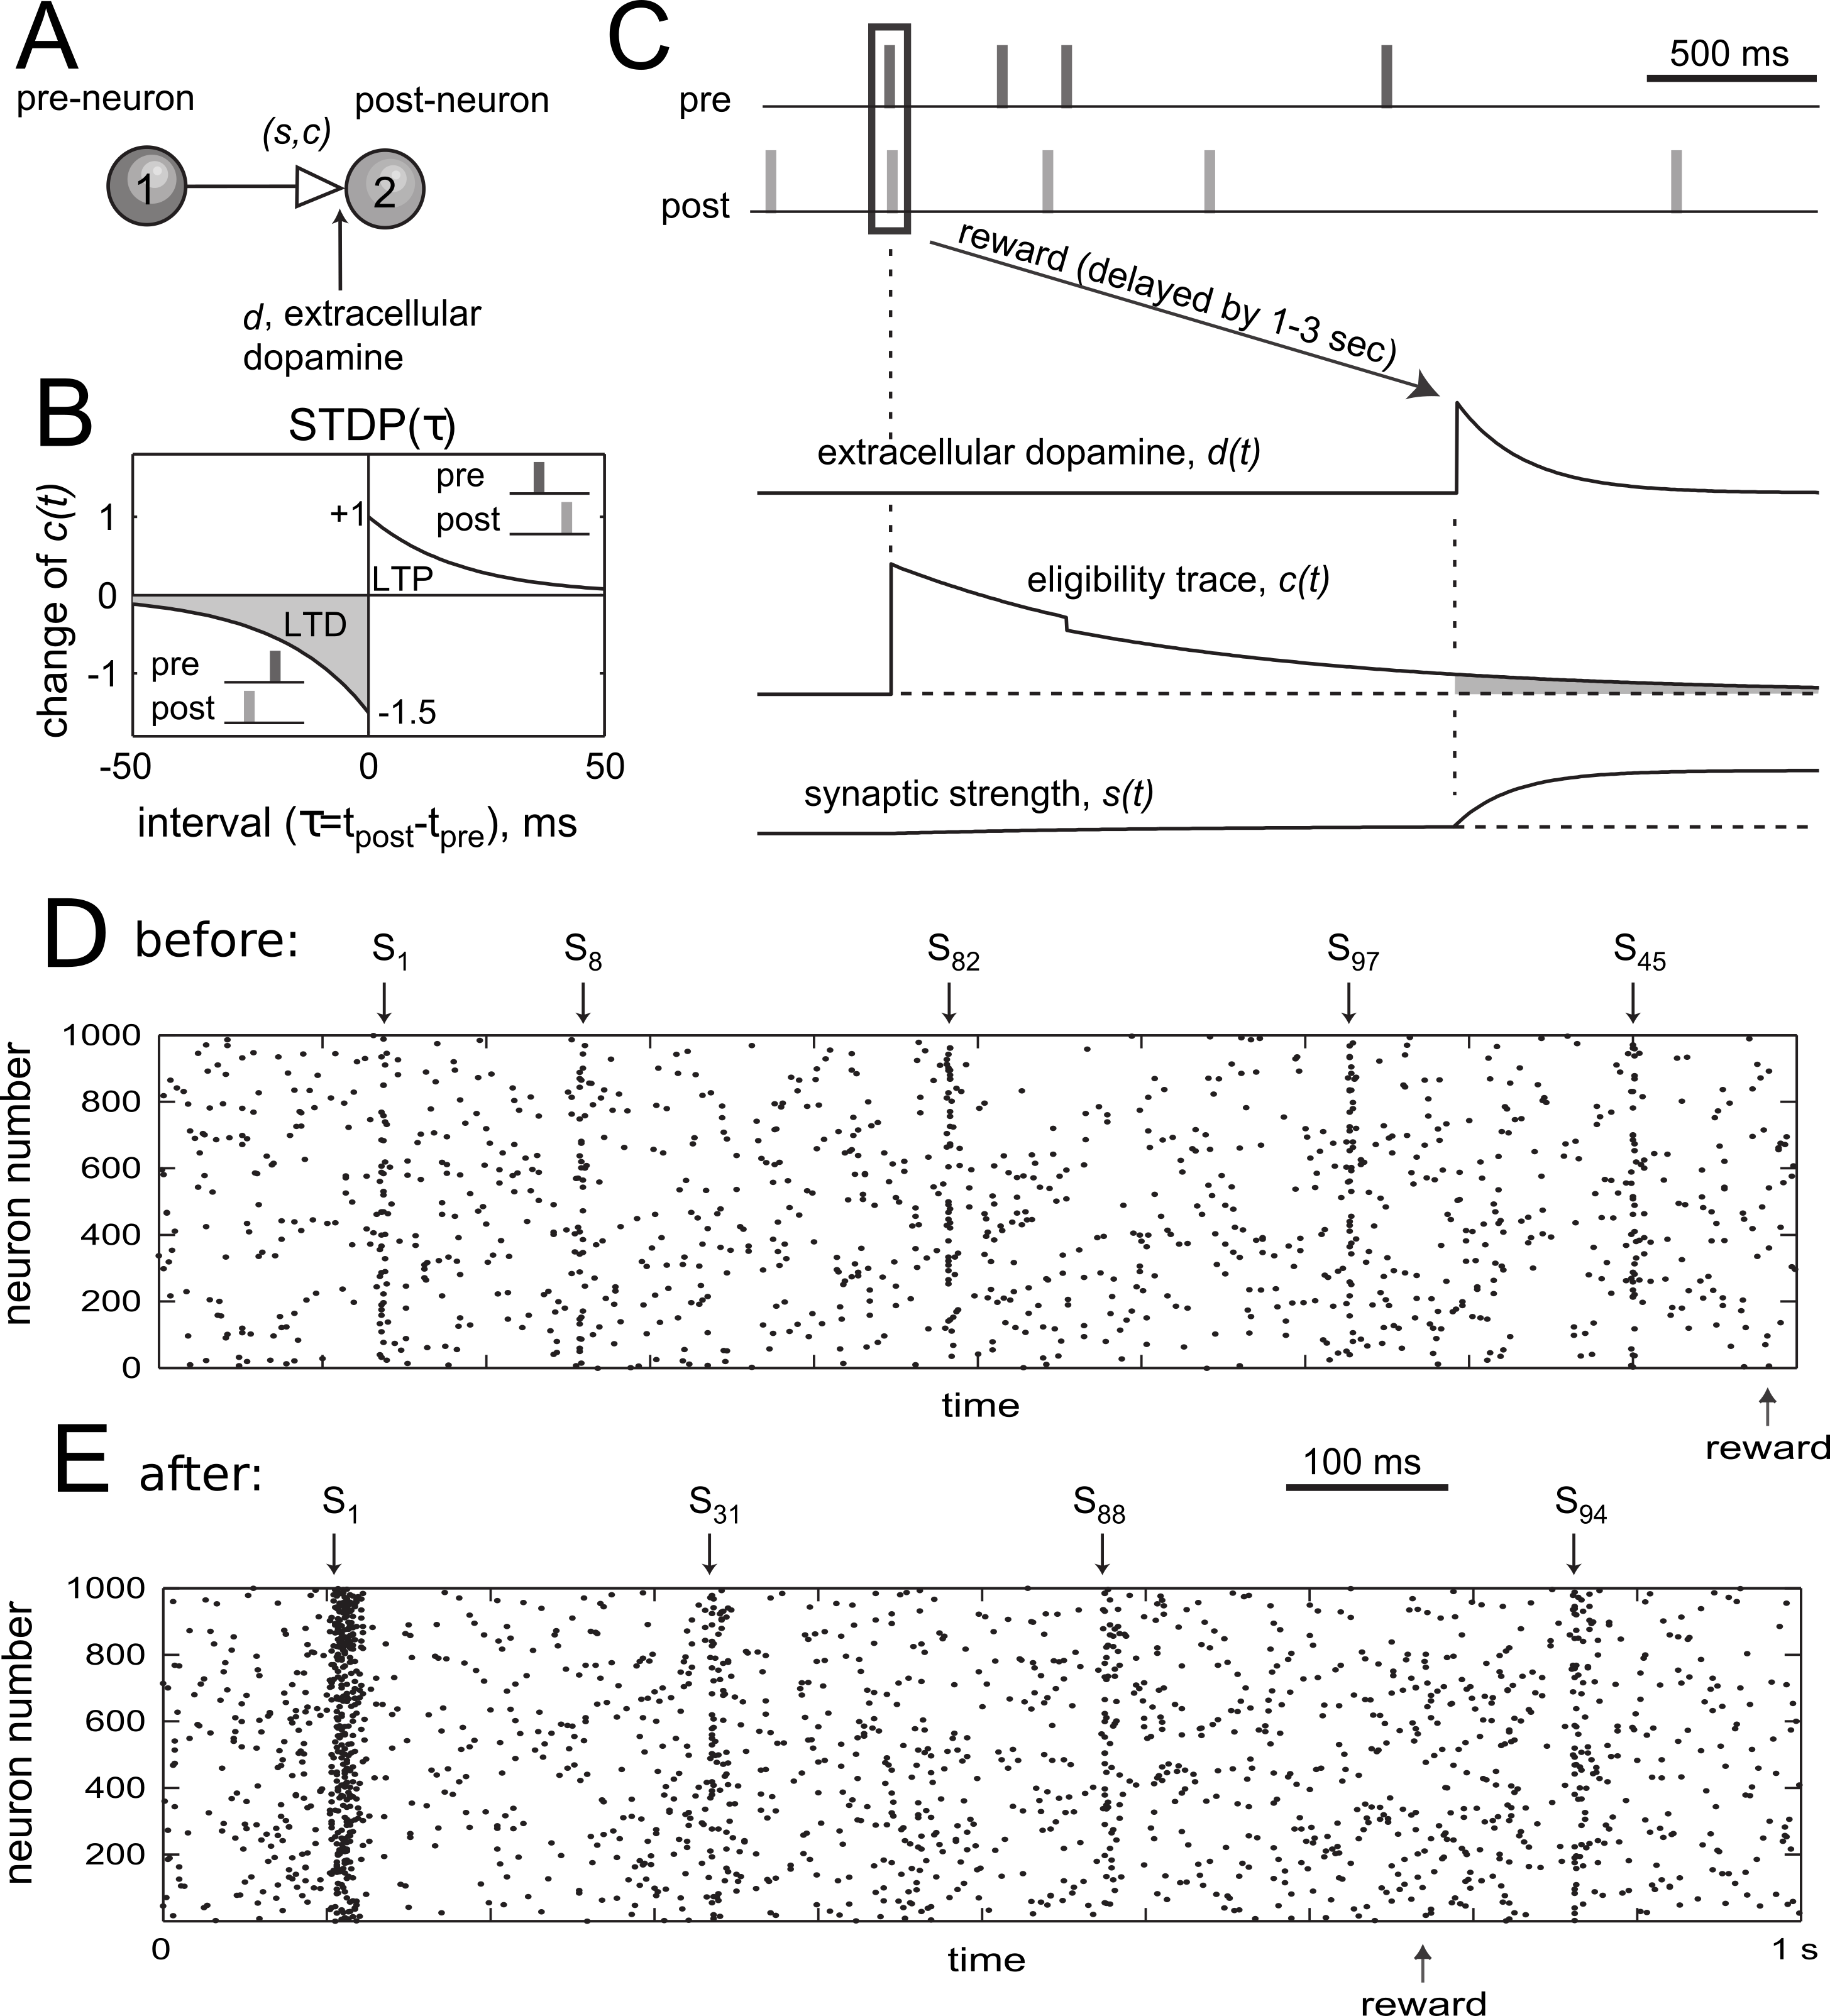
\includegraphics[width=12cm]{chapter1/figures/izhiIllustration/izhiIllustration.png}
        \caption[The Izhikevich proposal for a plasticity rule involving dopamine]{\textbf{According to Izhikevich's proposal, dopamine interacts with the classical STDP rule via eligibility traces.} (A) Illustration of the basic computational unit: a pre-post neuron pair with parameters holding the strength of the synapse between them (s) and the state of the eligibility trace (c). A third parameter (d) holds the level of extracellular dopamine. (B) A classical STDP rule is applied with regards to the timing of firing in the pre and post neurons to inform the eligibility trace rather than the synaptic strength. (C) Demonstration of the plasticity rule operating over a stretch of network activity. A pre-then-post firing event at a high temporal proximity causes an increase in the eligibility trace. Arrival of dopamine before the trace has completely decayed results in potentiation (increase in the parameter s). (D-E) Demonstration of how dopamine signalling can induce pathway specific plasticity despite operating as a volume signal. 100 different stimulation patterns are defined and applied continuously to the network. Only pattern S1 is consistently followed by a dopamine reward and is the only one to be potentiated. Adapted with permission from \cite{izhikevich2007solving}.}
        \label{fig:introduction:izhi}
    \end{figure}

    This Izhikevic thought experiment illustrates how a non-specific reward signal may interact with the activity and with established plasticity rules to reinforce just the parts of the circuit that are relevant for the task. It also highlights the importance of having a temporally narrow phasic signal to facilitate the selection of the correct synapses. Nevertheless, the mechanism suggested by Izhikevic as well as other proposals by computational neuroscientists \cite{fremaux2015neuromodulated} are all purely hypothetical and have not been established experimentally. This is mainly due to the absence of \textit{in vitro} systems that are able to control and monitor both the spiking activity in a neuronal circuit and the phasic neuromodulator signals applied to it. One such system has been recently proposed by Yagishita et. al. \cite{yagishita2014critical}. That system was based on a brain slice which includes both the main dopamine nucleus (VTA) and the striatum. The activity in the VTA was controlled via optogenetic activation, the spiking activity of specified striatal spiny neurons was controlled by directly patching them and specific synaptic spines were artificially activated by means of glutamate uncaging. This system was used to prove the hallmarks of the Izhikevic model, namely, that a synaptic activation coupled to an action potential in the post synaptic cell results in a potentiation only when followed by activation of the VTA within a stringent time window of about 1 second. Such slice based systems are indeed an attractive way to study the low level mechanisms by which neuromodulators interact with the activity and plasticity but they also suffer from a few drawbacks. Firstly, since they are based on a single tissue section they cannot incorporate more than a single neuromodulator nucleus into the same experiment and hence will not be able to investigate how different modulatory species, which are all important for plasticity and for the activity patterns in awake animals, interact with each other. Secondly, the slice system generates neuromodulatory pulses indirectly through stimulation of the relevant nucleus so they do not control the precise concentration of neuromodulator in the tissue, which has been shown to gate the plasticity in a non-trivial fashion \cite{otani2015dopaminergic}. In the next section we propose a culture based system that will address the experimental gaps.

    \label{sec:introduction:izi}

    \section{Proposed system and how it addresses present experimental gaps}
    To address the experimental shortcomings described above we propose to extend the established functionality of neuronal culture grown on MEAs with a rapid solution exchange functionality allowing application of neuromodulatory pulses onto an entire neuronal circuit at time scale of phasic volume transmission. As explained in the previous sections, both the latency in the pulse arrival and the its width are thought to be important parameters in the functioning of the neuromodulator system and for using it to achieve reinforcement learning. Thus it is crucial that the system allows for the agonist to arrive at the cells and be removed within no more than a few seconds. Such a functionality can only be supported by a neuronal culture and not by slices. The reason for this is that brain slices are normally \(150-300 \mu m\) thick so even if the solution around them were to be replaced very fast, additional diffusion into the tissue would be required which, given its thickness, would take more than a few seconds. In the case of neuronal culture, which forms a thin monolayer of no more than a few microns, such a diffusion bottleneck would not arise. An important part of the requirement is that the agonist pulse would span the entire culture as this spatial non-specificity is a conspicuous feature of the volume transmission process. Luckily, neuronal culture technology makes it far easier to restrict the tissue size in par with the requirements.

    The proposed system, if realized, would be able to readily employ any type of agonist or even combinations to test for interactions. Additionally, these experiments would be concentration-resolved because the extracellular solution would be directly manipulated. This aspect of the system would be useful if the precise agonist concentration values were to be of concern. A striking characteristic of the neuromodulator signalling is that, beyond the plasticity, it also elicits a direct effect on the activity in the target circuit. It is yet unknown how these seemingly distinct processes are coded for by the same neuromodulator species but it is plausible that the code has to do with tonic and phasic aspects of the signal which produce different agonist concentrations in the tissue. It is worthwhile to note that achieving rapid control over the extracellular chemistry could also be useful for studying intrinsic volume transmission processes. However, these processes are produced by localized secretion events within the tissue and therefore result in more spatially complex signals as compared to the extrinsic ones. Consequently, modelling intrinsic volume transmission might require a system that goes beyond simple solution exchange and allows generation also of spatially complex agonist patterns. Nevertheless, the system of concern here will hopefully serve as a proof-of-principle and hopefully pave the way for future more complex designs.

    Basing the system around neuronal culture would also provide access to the other advantages of the culture system which include, as described in section \ref{sec:introduction:achievements}, a growing ability to control the network architecture and to perform experiments over long stretches of time and thus allowing more complex learning paradigms to be explored. Finally, much of the theoretical computational studies, and especially those concerned with generic properties of neural circuits, employs simulated networks that are initially randomly connected (e.g., the above-mentioned Izhikevic model). Randomly organized neuronal cultures therefore comprise a natural experimental partner to these kinds of simulation data. In the next section we will review the technology that will be used to implement the rapid solution exchange.

    \section{Rapid solution exchange with microfluidics}
    Rapid solution exchange in neuroscience has been widely implemented via iontophoresis (e.g., \cite {jonas1993quantal,hestrin1992activation}). This application method ejects charged agonists from a tip of a micropipette by applying an electric potential to the fill solution. Although this technique is able to generate agonist transients at extremely fast time scales (sub millisecond), it is limited in its spatial scale and can only generate significant concentration increases around a single synapse or at most a single cell soma.

    The recent advent of microfluidic technology offers an exciting way for precision control over movement of liquid in an on-chip fluidic network. Microfluidic devices are typically fabricated with soft-lithography techniques (see section \ref{sec:methods:fabrication}) and consist of a network of flow channels each at the scale of several to hundreds of microns at most. The basis for the success of microfluidics is that the flow operates purely at the laminar flow regime. In macro-scale flow systems, due the larger dimensions and increased flow velocities, the internal inertial forces in the liquid greatly dominate the viscous ones and this results in a turbulent flow regime \cite{fluidBook}. This regime is characterized by localized turbulences, unexpected fluctuations and significant mixing between different parts of the liquid. The ratio between inertial and viscous influences is known as the Reynold's number (\(R_{e}\)) and turbulent flow occurs for \(R_{e}>10^{3}\). For lower \(R_{e}\), which is the case for microfluidic chips, the viscous influences dominate and the flow becomes smooth and predictable. In this regime, the flow forms separate liquid layers (lamina) which do not mix, hence the name laminar flow. Regardless of the input configuration, laminar flow always organizes in a simple axial configuration and is completely deterministic which allows the design of chips with programmatic routing and mixing of solute molecules and with accurate control of their spatiotemporal concentration profile. Most microfluidic systems are characterized by a particularly low Reynold's number, \(R_{e}<1\), which corresponds to the creeping flow regime. In this regime, the flow is well modeled by a version of the Navier-Stokes equations where the inertial term is completely neglected allowing simple analytical solutions. One important consequence of this is that the flow velocities in creeping flow always follow a parabolic profile which makes it easy to estimate shear stresses along the vertical axis.

    A renowned application of microfluidic technology is the flow focusing device \cite{takayama2001laminar}. This device comprises a main channel with three input ports in a fork-like design (i.e., they all share the same split point at the top of the main channel). The central input port carries an agonist molecule where as the side ports carry blank media. Because of the laminar flow, the streams originating from the different ports do not mix and the extent of diffusion that occurs between them as they proceed down the channel can by controlled via the flow velocity. By accurately adjusting the relative flow rates of the three streams the width of the central (agonist) one and its position across the channel may be accurately controlled. In this way, the agonist can be applied to very specific locations with subcellular resolution. Such subcellular localization is similar in performance to iontophoretic application. However, in contrast to iontophoresis, this approach may be readily adapted to larger tissues as the scales merely depend on the device geometry and on the flow rates and how they are controlled. This is the basis for our agonist pulsing device, described next.

    This Ph.D work will utilize a y-shaped (2 input ports) microfluidic device with one port carrying the agonist and one carrying blank media. At baseline, the flow rate of the blank stream will be significantly higher than that of the agonist stream so the latter will be restricted to a small side section. When a pulse command is issued, the flow rates will be temporarily flipped so that the agonist stream will be pushed across the channel in place of the diminished blank stream. When the flow rates switch back, the streams will revert back to the baseline arrangement but this will result in an agonist pulse traveling along the channel and in a temporary exposure of the cells to it (figure \ref{fig:introduction:intShift}). Such sweeping back and forth of a flow stream is termed interface shifting \cite{bae2009rapid}. In this way agonist pulses can be generated that encompass practically the entire channel cross section. In chapter \ref{chap:microculturePulses} we will show that this approach may be used to successfully mimic the temporal exposure profiles of phasic neuromodulator signalling. This application of microfluidics to neuronal studies highlights the great potential that this technology holds for neuroscience questions that involve extracellular species. Nevertheless, microfluidic applications to neuroscience, and in particular those involving flow, are still at their infancy, as reviewed in the next section.

        \begin{figure}[!htb]
        \centering
        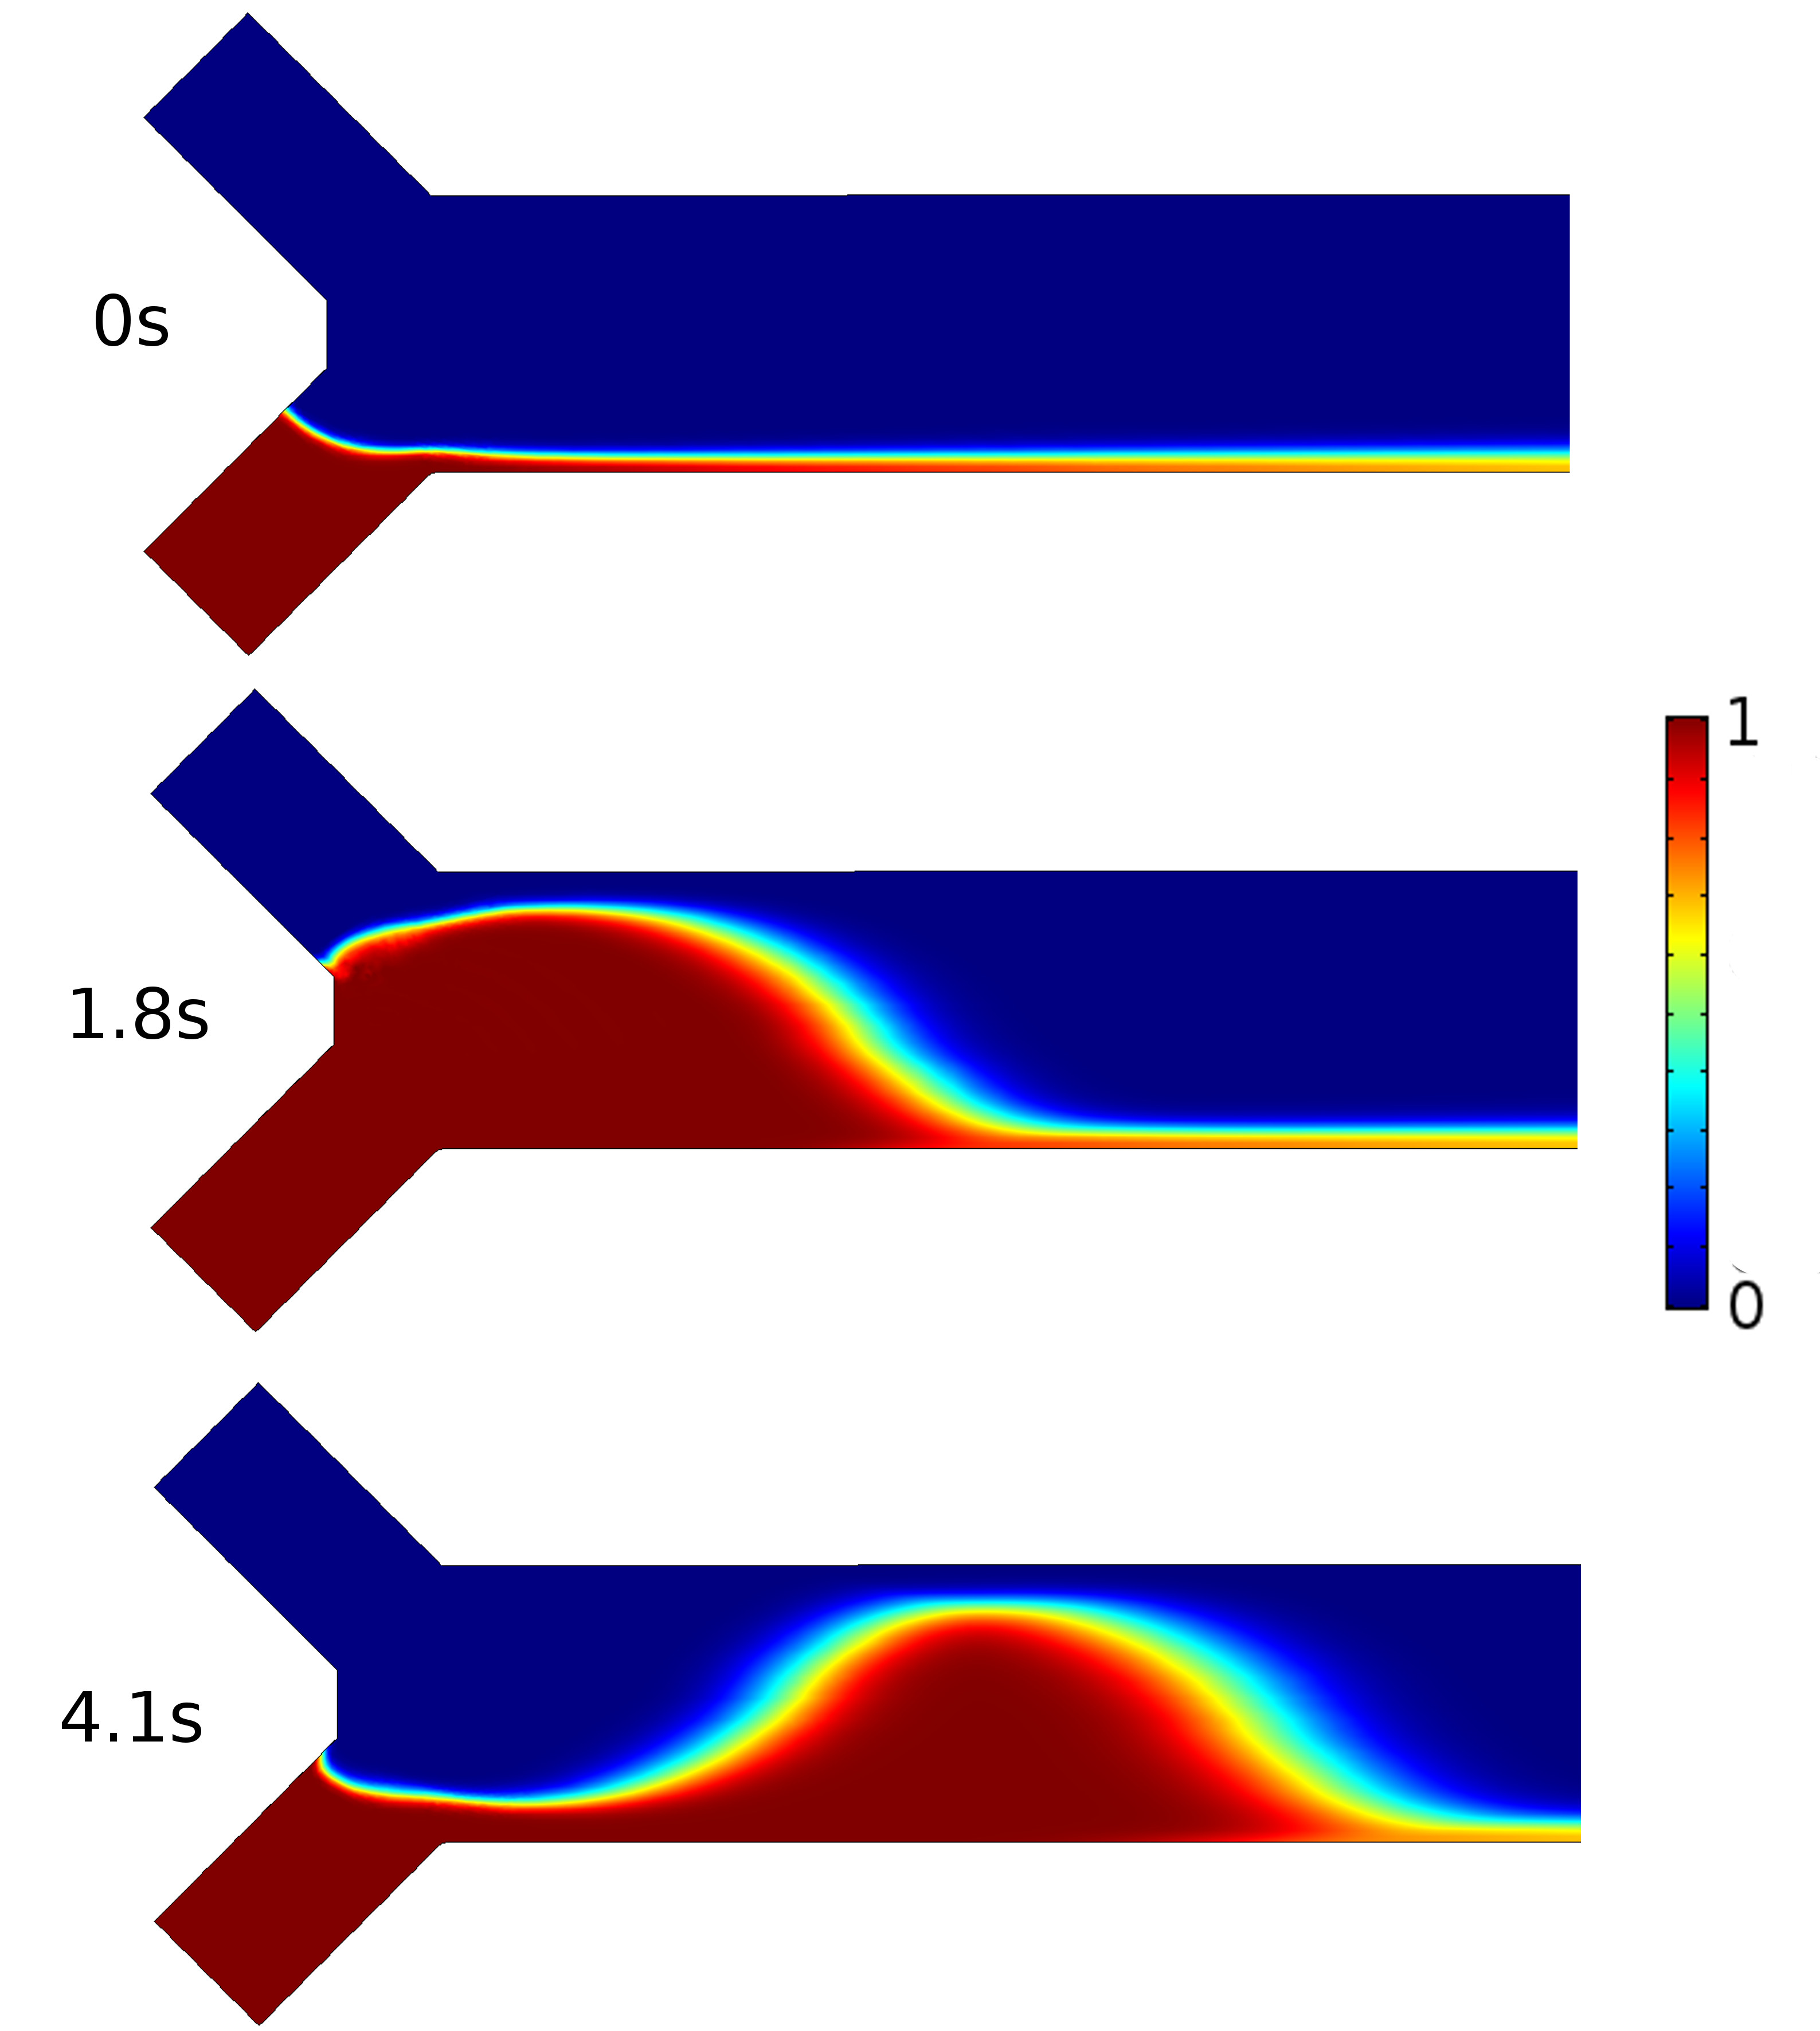
\includegraphics[width=12cm]{chapter1/figures/intShift/intShift.jpg}
        \caption[Generating a pulse with the interface shifting method]{\textbf{Flipping between the flow rates in the input ports generates an agonist pulse.} Red color depicts the agonist stream whereas the blue depicts the blank stream. Flow rates are initially unbalanced in favour of the blank stream but flipped momentarily upon a pulse command. This results in sweeping of the interface back and forth and generating of an agonist pulse travelling down the channel. These images were produced by a finite element simulation used to characterize the pulsing performance in chapter \ref{chap:microculturePulses}. Color scale shows normalized concentration (1 in agonist stream and 0 in the blank stream).}
        \label{fig:introduction:intShift}
    \end{figure}
    \label{sec:introduction:mufdDrugDelivery}

    \subsection{Microfluidics in neuroscience}
    Microfluidics technology has sprung into the neuroscience psyche with the introduction of the innovative compartmentalized culture system by Taylor et. al. \cite{taylor2005microfluidic}. Taylor's device, a.k.a. `Taylor's ladder', comprises two large scale compartments that are connected by small rectangular tunnels which are only \(1 \mu m\) high and wide. A neuronal culture seeded into one of the compartments are constrained to that side because the tunnels are too small for cell somata to go through. Axons, however, are able to traverse the tunnels by virtue of their smaller dimensions and so, after a few days, the unseeded compartment become inhabited with axons only. This arrangement allows pharmacological and molecular biology assays to be conducted only on the axons. This unique compartmentalization of neurons has enabled breakthrough research into the localization of biological markers within the neuron with important consequences to cell signalling and developmental neurobiology. This work demonstrates the major usefulness of microfluidic technology in achieving topological control and was extended by many others. These further work include compartmentalization of synapses \cite{taylor2010microfluidic}, of co-cultures \cite{robertson2014chemically,renault2015combining} and even of multiple cell populations with directional connectivity between them \cite{peyrin2011axon,honegger2016microfluidic,dauth2016neurons}. Evidently, the compatibility of microfluidic devices with neuronal culturing has been well established but also found to be more challenging than in standard conditions due to the involved materials and the imposed chamber geometries \cite{millet2007microfluidic}.


    \label{sec:introduction:mufdNeuroscience}
    \subsection{Neurons and flow}
    The above-mentioned neuroscience applications mainly utilized the fact that microfluidic technology involves rapid prototyping of micro-structures with bespoke designs. However, the main aspect of the technology, rapid and precise fluid and solute handling, has hardly been tapped as far as neuroscience applications are concerned. This despite the potential of such applications to study aspects of the neuronal volume transmission. A likely cause for this disregard is probably that neurons are considered to be extremely sensitive to mechanical perturbations and to shear stress, so such experiments might be expected to be difficult. Indeed some of the studies that did employ microfluidic flow incorporated shear protection measures to try and circumvent this issue \cite{wang2008microfluidics,morel2012amplification}. These studies were indeed able to perform elegant experiments involving generation of growth factor gradients around developing neurons to attract or repel their growth cones. However, they did not show data to demonstrate that the shear protection was required and seemed to take its necessity for granted. Another recent work seemed to contradict the shear sensitivity notion as it reported that primary rat neurons may be subjected to very high shear for over 24 hours without adverse effects \cite{liu2013galanin}. Overall, the effect of shear stress on the function and viability of neuronal culture has not been systematically studied and is poorly understood. Nevertheless, understanding the shear limitations is critical if the full potential of flow microfluidics is to be realised for neuroscience studies. In this context, it is important to mention some reports of neurons developing for long term in culture under very slow gravity fed microfluidic flow, where the magnitude of convection is comparable to diffusion so shear is not a factor \cite{choi2013neurotoxic,millet2007microfluidic,kumamoto2015effects}. This Ph.D work is concerned with much faster flow rates and will provide novel data regarding the viability of neuronal culture in such conditions. Additionally, all the above-reported work did not included any kind of electrophysiology under flow so it is altogether unknown how it affects the network activity. Possible influences could involve activation of stretch receptors or interaction with intrinsic volume transmission processes in the tissue. Thus, the inclusion of micro electrode arrays in the system proposed here will also serve to provide novel data regarding the spiking network activity under flow.
    \label{sec:introduction:neuroFlow}

    \section{Ph.D objectives}
    In the preceding sections, we identified gaps in current \textit{in vitro} neuroscience experimental platforms given recent developments in neuromodulator signalling. To address these gaps we proposed a system combining the technologies of neuronal culture, microelectrode arrays microfluidics. We further described the state of the art of these technologies and the technical hurdles that still need to be overcome. Thus, we are now in position to define the goals of this Ph.D work. The main goal is the development of a system for rapid solution exchange to an entire neuronal culture at time scales matching phasic neuromodulator signalling with a concurrent measurement and control of network spiking activity. To achieve this goal we will traverse 4 subgoals accounting for the main technical steps that need to be ascended. These subgoals match the experimental chapters of this thesis:

    \begin{enumerate}
    \item Establish gold standard neuronal culture recording and stimulation using MEAs. In this chapter we will also attempt to induce plasticity in the network in conjunction with slow bath application of dopamine. This will serve as motivation for the further integration with microfluidics.

    \item Establish a long term neuronal culture in microfluidic devices at the desirable geometry and assess its viability under the required flow rates.

    \item Characterize the stability of the spontaneous and evoked network activity under flow at the required flow rates.

    \item Combine all the lessons learned in the previous steps to build a working prototype of rapid solution exchange to an entire neuronal culture at the time scales of phasic neuromodulator signalling. Demonstrate the functionality of model by pulsing dopamine in conjunction with applying stimulations to the network.
    \end{enumerate}


    \label{sec:introduction:objs}

